\documentclass[fleqn]{article}
\author{MODFLOW Development Team}

\usepackage{amsmath}
\usepackage{xcolor}
\usepackage{graphicx}
\graphicspath{{./figures/}}


\begin{document}

\title{Surface Water Flow in MODFLOW 6}
\maketitle

\tableofcontents

\section{Introduction}
The Surface Water Flow (SFW) Model simulates one-dimensional channel flow and two-dimensional overland flow.  The SWF Model is a new model type in the MODFLOW 6 framework.  Like other models in the MODFLOW 6 framework, the SWF Model consists of required and optional packages.

\subsection{Mathematical Model}
Following~\cite{panday2004} and~\cite{hughes2012documentation} The diffusive wave approximation to the full St. Venant equations can be expressed as

\begin{equation}
  \frac{\partial A}{\partial t} +
  \frac{\partial}{\partial \ell}
  \left (
  \frac{A R^{\frac{2}{3}}}{n \left | \frac{\partial h}{\partial \ell} \right |^{\frac{1}{2}} } \frac{\partial h}{\partial \ell}
  \right )
  + A q_{\ell}
  = 0
  \label{eqn:onedpd}
\end{equation}

\noindent for one-dimensional channel flow or as

\begin{equation}
  \frac{\partial h}{\partial t}
  + \frac{\partial}{\partial x}
  \left (
  \frac{d^{\frac{5}{3}}}{n \left | \frac{\partial h}{\partial s} \right |^{\frac{1}{2}} } \frac{\partial h}{\partial x}
  \right )
  + \frac{\partial}{\partial y}
  \left (
  \frac{d^{\frac{5}{3}}}{n \left | \frac{\partial h}{\partial s} \right |^{\frac{1}{2}} } \frac{\partial h}{\partial y}
  \right )
  + d q_s
  = 0
  \label{eqn:twodpd}
\end{equation}

\noindent for two-dimensional overland flow.  In equation~\ref{eqn:onedpd}, $\ell$ is the coordinate direction along the stream channel.  In equation~\ref{eqn:twodpd}, $x$ and $y$ are the two-dimensional coordinate directions. In both equation~\ref{eqn:onedpd} and equation~\ref{eqn:twodpd} $A$ is the cross-sectional area ($L^2$) for flow, $t$ is time ($T$), $s$ is the direction along the channel, $R$ is the hydraulic radius ($L$), $n$ is the Mannings roughness coefficient ($T/L^{\frac{1}{3}}$), $q_{\ell}$ is a source or sink term, in dimensions of $1/T$, representing the volume of water per unit volume of channel per unit time, $h$ is the water surface elevation ($L$) defined as the depth of water $d$ above the channel bottom elevation $z$ ($d = h - z$), and $q_s$ is a source and sink term, in dimensions of $1/T$, representing the source or sink volume of water per unit volume per unit time.

\section{Spatial Discretization}
The SWF Model supports two different types of discretization approaches: a one-dimensional channel network and a two-dimensional structured or unstructured overland flow grid.  A SWF Model must use one or the other discretization approach.  

\subsection{One-Dimensional Channel Network}

A one-dimensional channel network is represented using the Discretization by Lines (DISL) Package.  

\begin{figure}
\centering
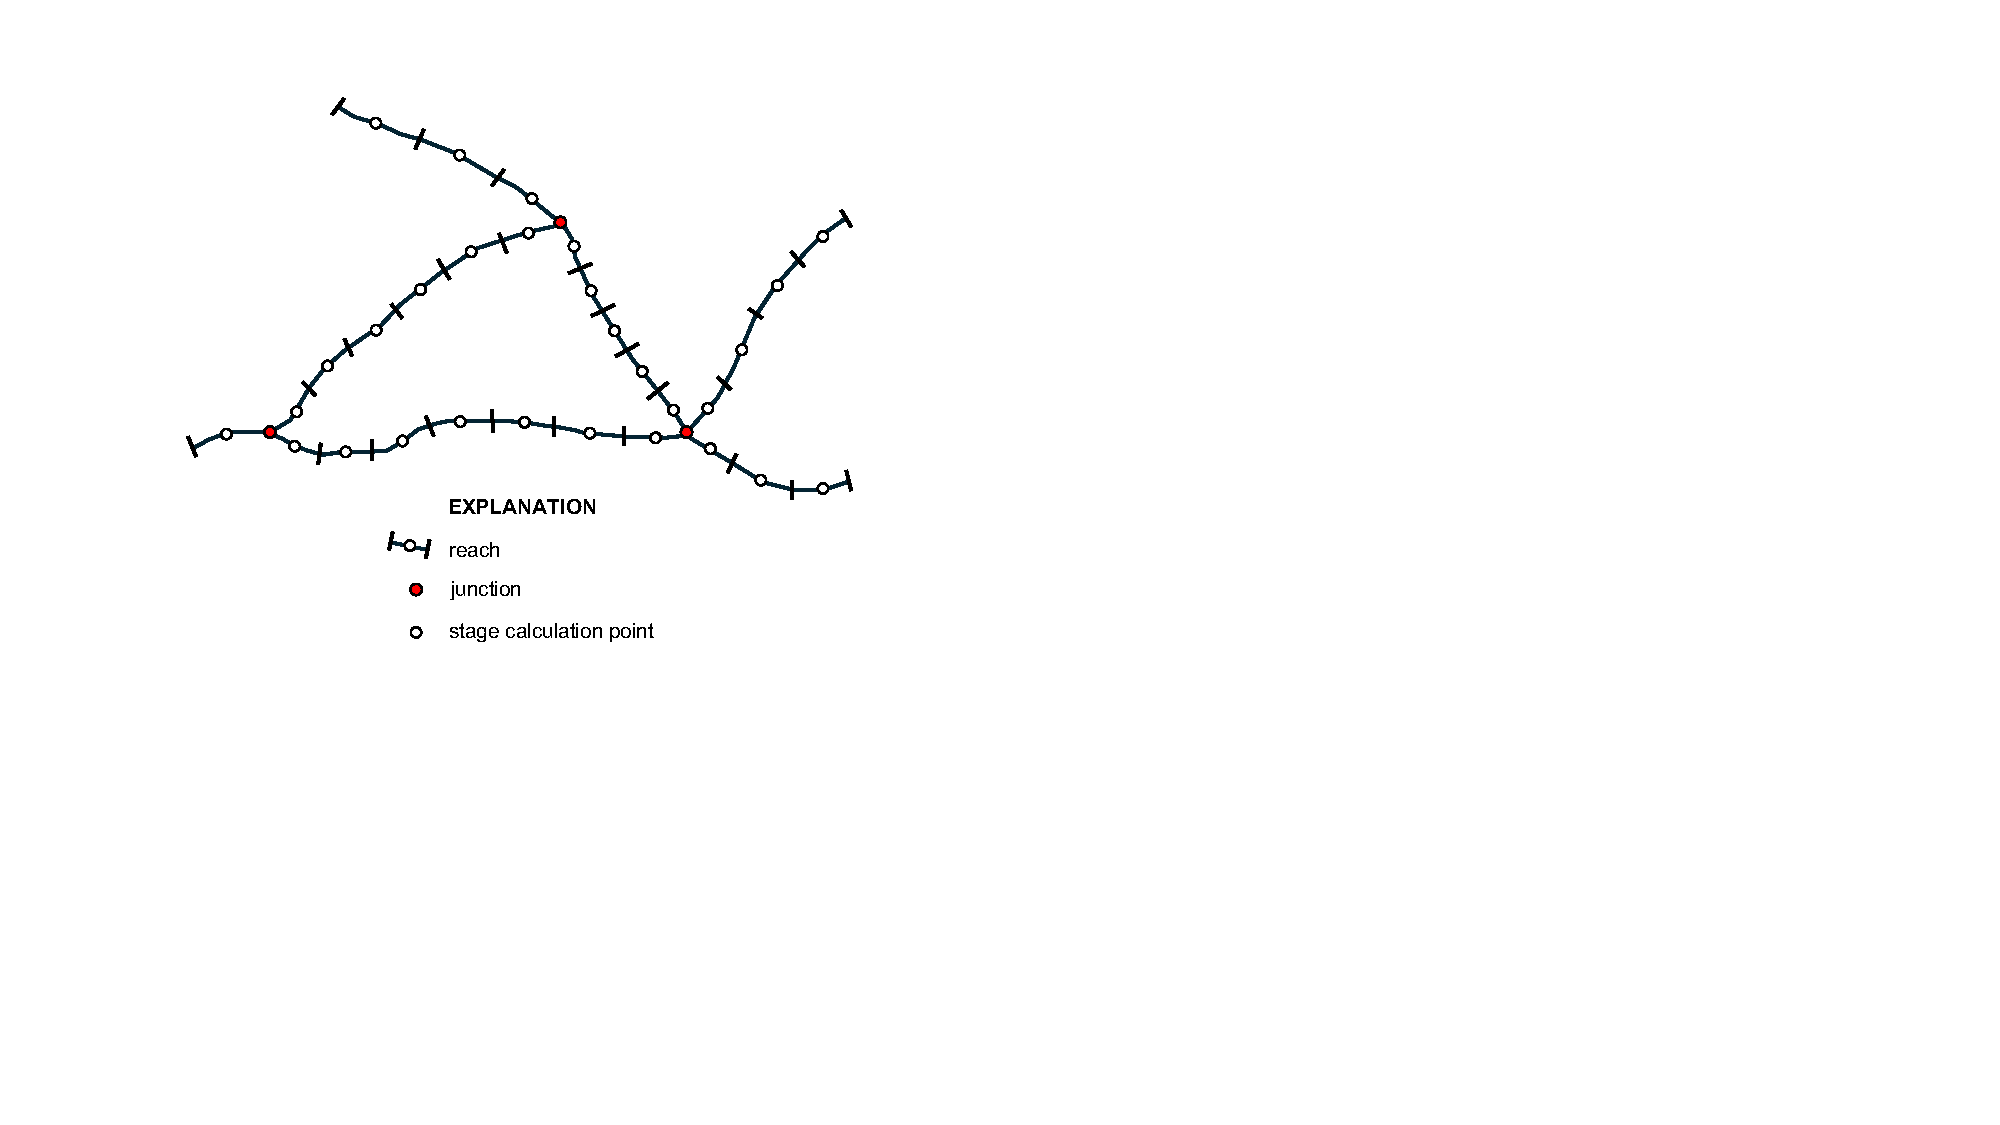
\includegraphics[scale=0.9]{figures/channel_network.pdf}
\caption[Schematic showing a channel network.]{Schematic showing a channel network.  The channel network is discretized by the user into computational elements called reaches.  Stage is calculated within the reach at stage calculation points.  Stage calculations are typically located halfway between the reach start and reach end vertices, however, the user can adjust the fractional position of the stage calculation point along the reach.}
\label{fig:channel_network}
\end{figure}

\subsection{Two-Dimensional Overland Flow}
Two-dimensional overland flow can be represented using either the regular structured grid discretization (DIS) Package or the unstructured discretization by vertices (DISV) Package.  

\subsection{Channel Cross Sections}

\section{Numerical Solution}

\subsection{Newton-Raphson Method}

Flow throughout the connected channel network is based on a Newton-Raphson formulation, in which the following equation is formulated and solved simultaneously for each reach \textcolor{red}{change n and m to i and j?}

\begin{equation}
\label{eqn:nr-cvfd}
\begin{split}
\left ( \sum\limits_{m \in \eta_{n}} \frac{\partial Q_{n,m}}{\partial h_n} + \frac{\partial Q_{n,s}}{\partial h_n} - \frac{\partial Q_{STO}}{\partial h_n} \right ) h^k_n + 
\sum\limits_{m \in \eta_{n}} \frac{\partial Q_{n,m}}{\partial h_m} h^k_{m} = \\
- \left ( \sum\limits_{m \in \eta_{n}} Q_{n,m} + Q_{n,s} - Q_{STO} \right ) + \\
\left ( \sum\limits_{m \in \eta_{n}} \frac{\partial Q_{n,m}}{\partial h_n} + \frac{\partial Q_{n,s}}{\partial h_n} - \frac{\partial Q_{STO}}{\partial h_n} \right ) h^{k-1}_n + \sum\limits_{m \in \eta_{n}} \frac{\partial Q_{n,m}}{\partial h_m} h^{k-1}_{m}.
\end{split}
\end{equation}

\subsection{Discretized Flow Expression}

Manning's equation is written as

\begin{equation}
  Q = \frac{1}{n} A R^{\frac{2}{3}} \sqrt{S_f}
\end{equation}

\noindent where $R$ is the hydraulic radius equal to $A / P$.  For the numerical implementation in MODFLOW we express Manning's equation as a product of a conductance term and the head difference between reach $n$ and $m$:

\begin{equation}
  Q_{nm} = C_{nm} \left ( h_m - h_n \right ).
\end{equation}

\noindent The conductance-based flow expression was selected so that individual conductances can be calculated for two connected reaches and then averaged together to give the conductance for the connection.  The average conductance between reach $n$ and reach $m$ ($C_{nm}$) is calculated by averaging a conductance for reach $n$ with a conductance for reach $m$.  The conductance for reach $n$, from the stage calculation point to the shared face with reach $m$, is denoted by $C_{n \rightarrow | m}$ and has dimensions of $L^2/T$.  The conductance for reach $m$, in the direction of reach $n$, is denoted by $C_{m \rightarrow | n}$ and also has dimensions of $L^2/T$.

The average conductance between reach $n$ and reach $m$ is calculated using the harmonic mean of $C_{n \rightarrow | m}$ and $C_{m \rightarrow | n}$ to give

\begin{equation}
  C_{nm} = \frac{C_{n \rightarrow | m}  C_{m \rightarrow | n}}{C_{n \rightarrow | m} + C_{m \rightarrow | n}}.
\end{equation}

\noindent The harmonic mean preferentially weights the average toward the lower of the two values and is based on piecewise constant reach properties that may change abruptly at the face between different reaches.

The conductance for reach $n$ in the $m$ direction ($C_{n \rightarrow | m}$) can be expressed as

\begin{equation}
  C_{n \rightarrow | m} = 
  \frac{
  A_n 
  R_{n}^{\frac{2}{3}}
  }
  {n_n
  L_{n \rightarrow | m}
  \sqrt{| \gamma_n |}
  },
\label{eqn:cn}
\end{equation}


%\begin{equation}
%  C_{n \rightarrow | m} = 
% \frac{A_n R_{n}^{\frac{2}{3}}}{n_n}
% \frac{1}{L_{n \rightarrow | m}}
% \frac{1}{ \sqrt{ \frac{ | \left ( h_m - h_n \right ) | } {L_{nm}}} }
%  \frac{1}{\sqrt{| \gamma_n |}}
%\end{equation}

%\begin{equation}
%  C_{n \rightarrow | m} = \frac{B_n}{ L_{nm} \sqrt{ \frac{ | \left ( h_m - h_n \right ) | } {L_{nm}}} }
%\end{equation}

\noindent where $A_n$ is the cross-sectional flow area ($L^2$) for reach $n$ calculated as a function of the water depth, $R_n$ is the hydraulic radius ($L$) for reach $n$, which is the cross-sectional flow area divided by the wetted perimeter, calculated as a function of the water depth, $n_n$ is the Manning's roughness coefficient ($T/L^{\frac{1}{3}}$) for reach $n$,  $L_{n \rightarrow | m}$ is the distance ($L$) from the stage calculation point to the shared edge between reach $n$ and $m$, and $\gamma_n$ is the hydraulic gradient ($L^0$) for reach $n$.

Several of the terms in equation \ref{eqn:cn} are combined into a single term for reach $n$ called channel conveyance ($B_n$), which is defined as

\begin{equation}
  B_n = \frac{A_n R_n^{\frac{2}{3}}}{n_n}.
\label{eqn:conveyance}
\end{equation}

\noindent Channel conveyance for reach $n$ is calculated as a function of an upstream-weighted water depth.  Thus, channel conveyance for reach $n$ can be written as

\begin{equation}
  B_n = \frac{A_n (d_u) R_n (d_u) ^{\frac{2}{3}}}{n_n},
\label{eqn:conveyancedu}
\end{equation}

\noindent where the $A_n$ and $R_n$ terms include $(d_u)$ to indicate that they are calculated as a function of $d_u$.  $d_u$ is assigned to the depth of the reach (either $n$ or $m$) with the higher stage:

\[
d_u = 
\begin{cases}
  d_n & \text{if $h_n>h_m$} \\
  d_m & \text{otherwise}
\end{cases}.
\]

With this definition for channel conveyance, equation \ref{eqn:cn} can be simplified as

\begin{equation}
  C_{n \rightarrow | m} = 
  \frac{
  B_n 
  }
  {
  L_{n \rightarrow | m}
  \sqrt{| \gamma_n |}
  },
\label{eqn:cn2}
\end{equation}

Channel conveyance is calculated in several different ways depending on how a cross section is defined for a reach.  For the cross sections shown in figure \ref{fig:cxs} a single Manning's roughness coefficient is assigned for the entire section.  If a single Manning's roughness coefficient is used to define the entire section for reach $n$, then the channel conveyance is calculated according to equation \ref{eqn:conveyance}.  If a cross section does not have a constant Manning's roughness coefficient for all line segments that define the channel, as shown for example in Figure \ref{fig:cxs_rough}, then a composite conveyance is calculated by summing the individual conveyance parts for the channel as

\begin{equation}
  B_n = \sum_{i=1}^{NLS} \frac{A_{n,i} \left ( \frac {A_{n,i}}{P_{n,i}}\right )^{\frac{2}{3}}}{n_{n,i}},
\end{equation}

\noindent where $NLS$ is the number of line segments used to define the channel cross section.

% This figure below is for the case where roughness is the same for every line segment in the cross section 
\begin{figure}[h!tbp]
	\centering
	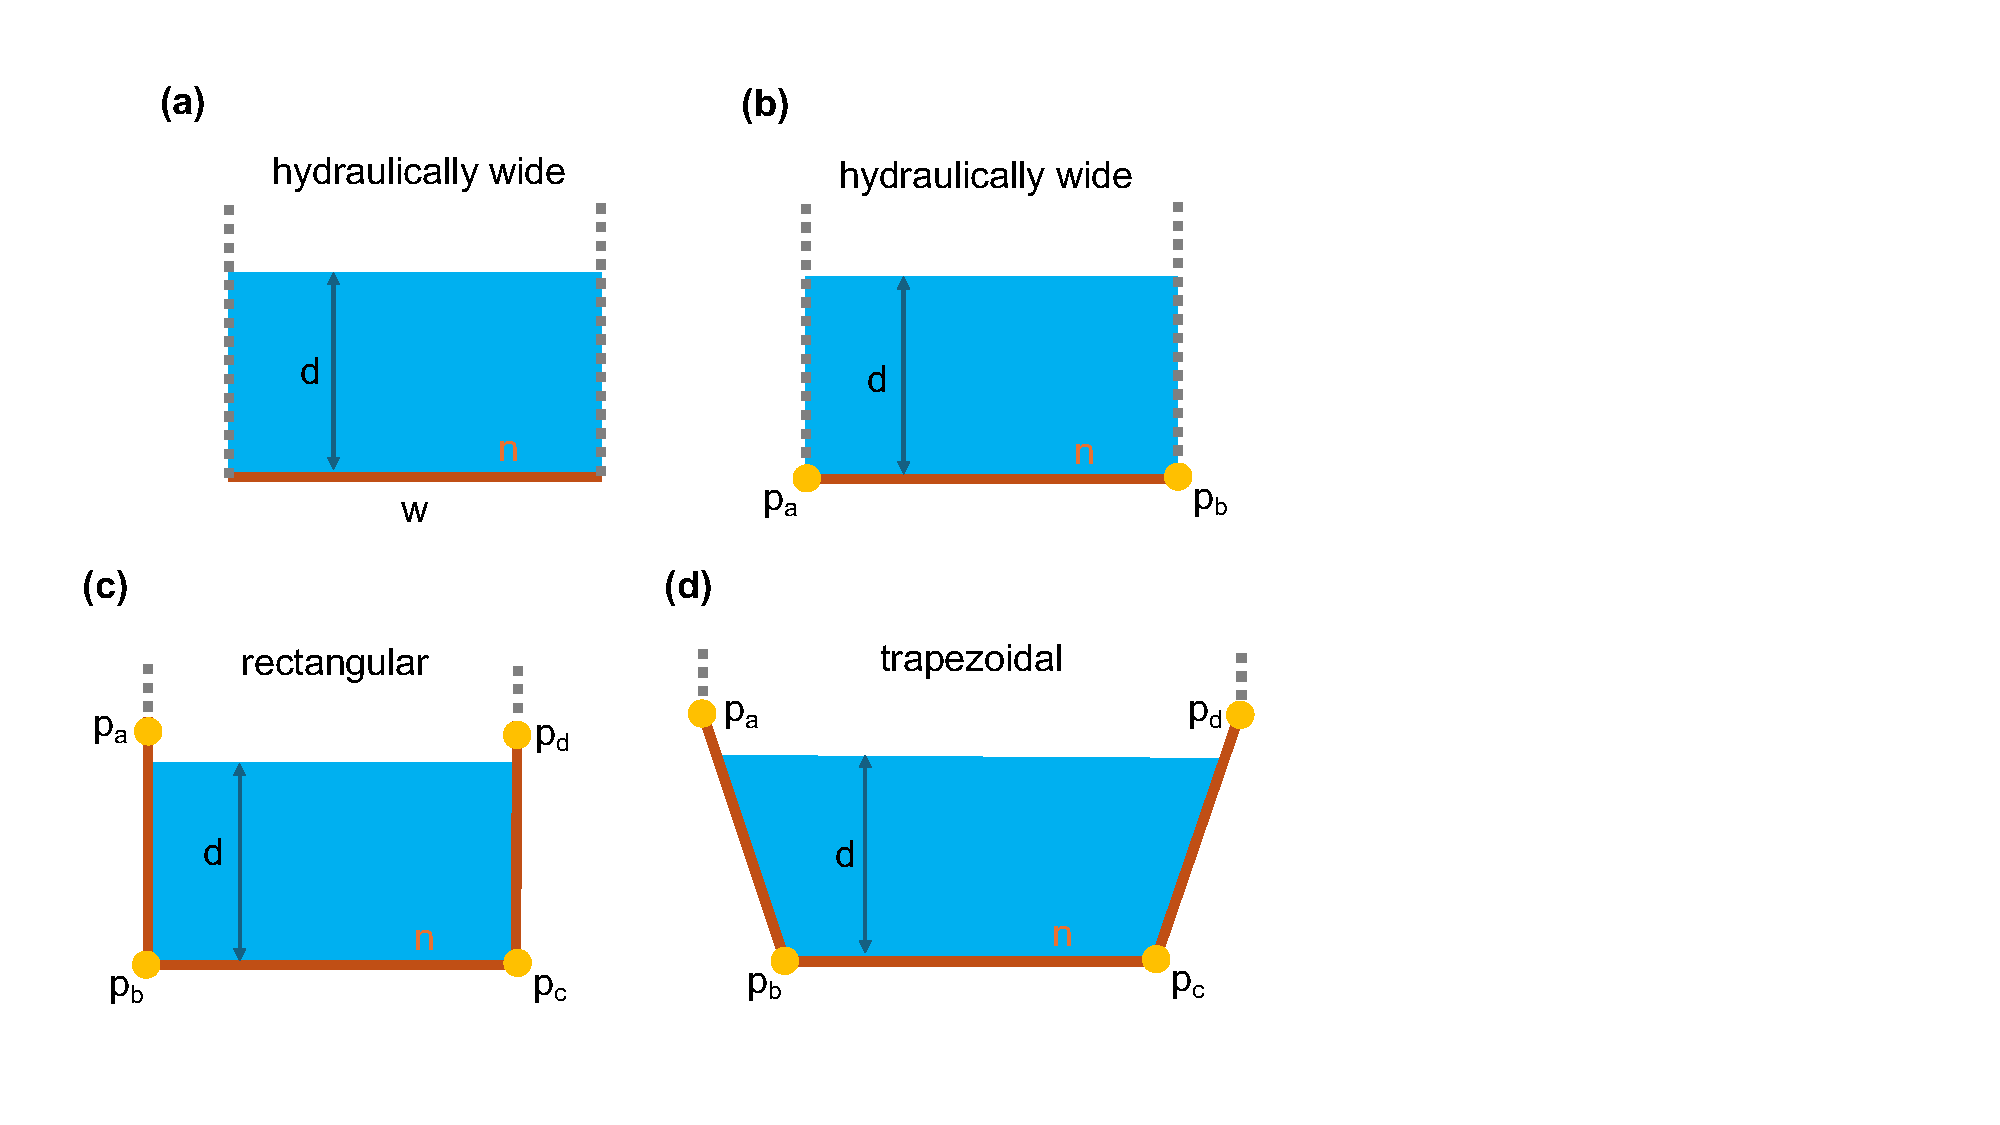
\includegraphics[scale=0.5]{figures/cxs.pdf}
	\caption[Schematic showing different types of channel cross sections with constant roughness.]{Schematic showing different types of cross sections with a single Manning's roughness coefficient $n$: (a) hydraulically wide cross section defined using the width input parameter; (b) hydraulically wide cross section defined using two points; (c) a rectangular cross section defined using four points, and (d) a trapezoidal cross section defined using four points.  For the hydraulically wide rectangular cross sections in (a) and (b) the model does not include any channel resistance for the vertical wetted sections corresponding to the dashed lines.  For cross sections shown in (c) and (d), if the water surface rises above the channel points, no channel resistance is included for sections above the uppermost points}
	\label{fig:cxs}
\end{figure}

% This figure below is for the case where roughness varies for each line segment in the cross section 
\begin{figure}[h!tbp]
	\centering
	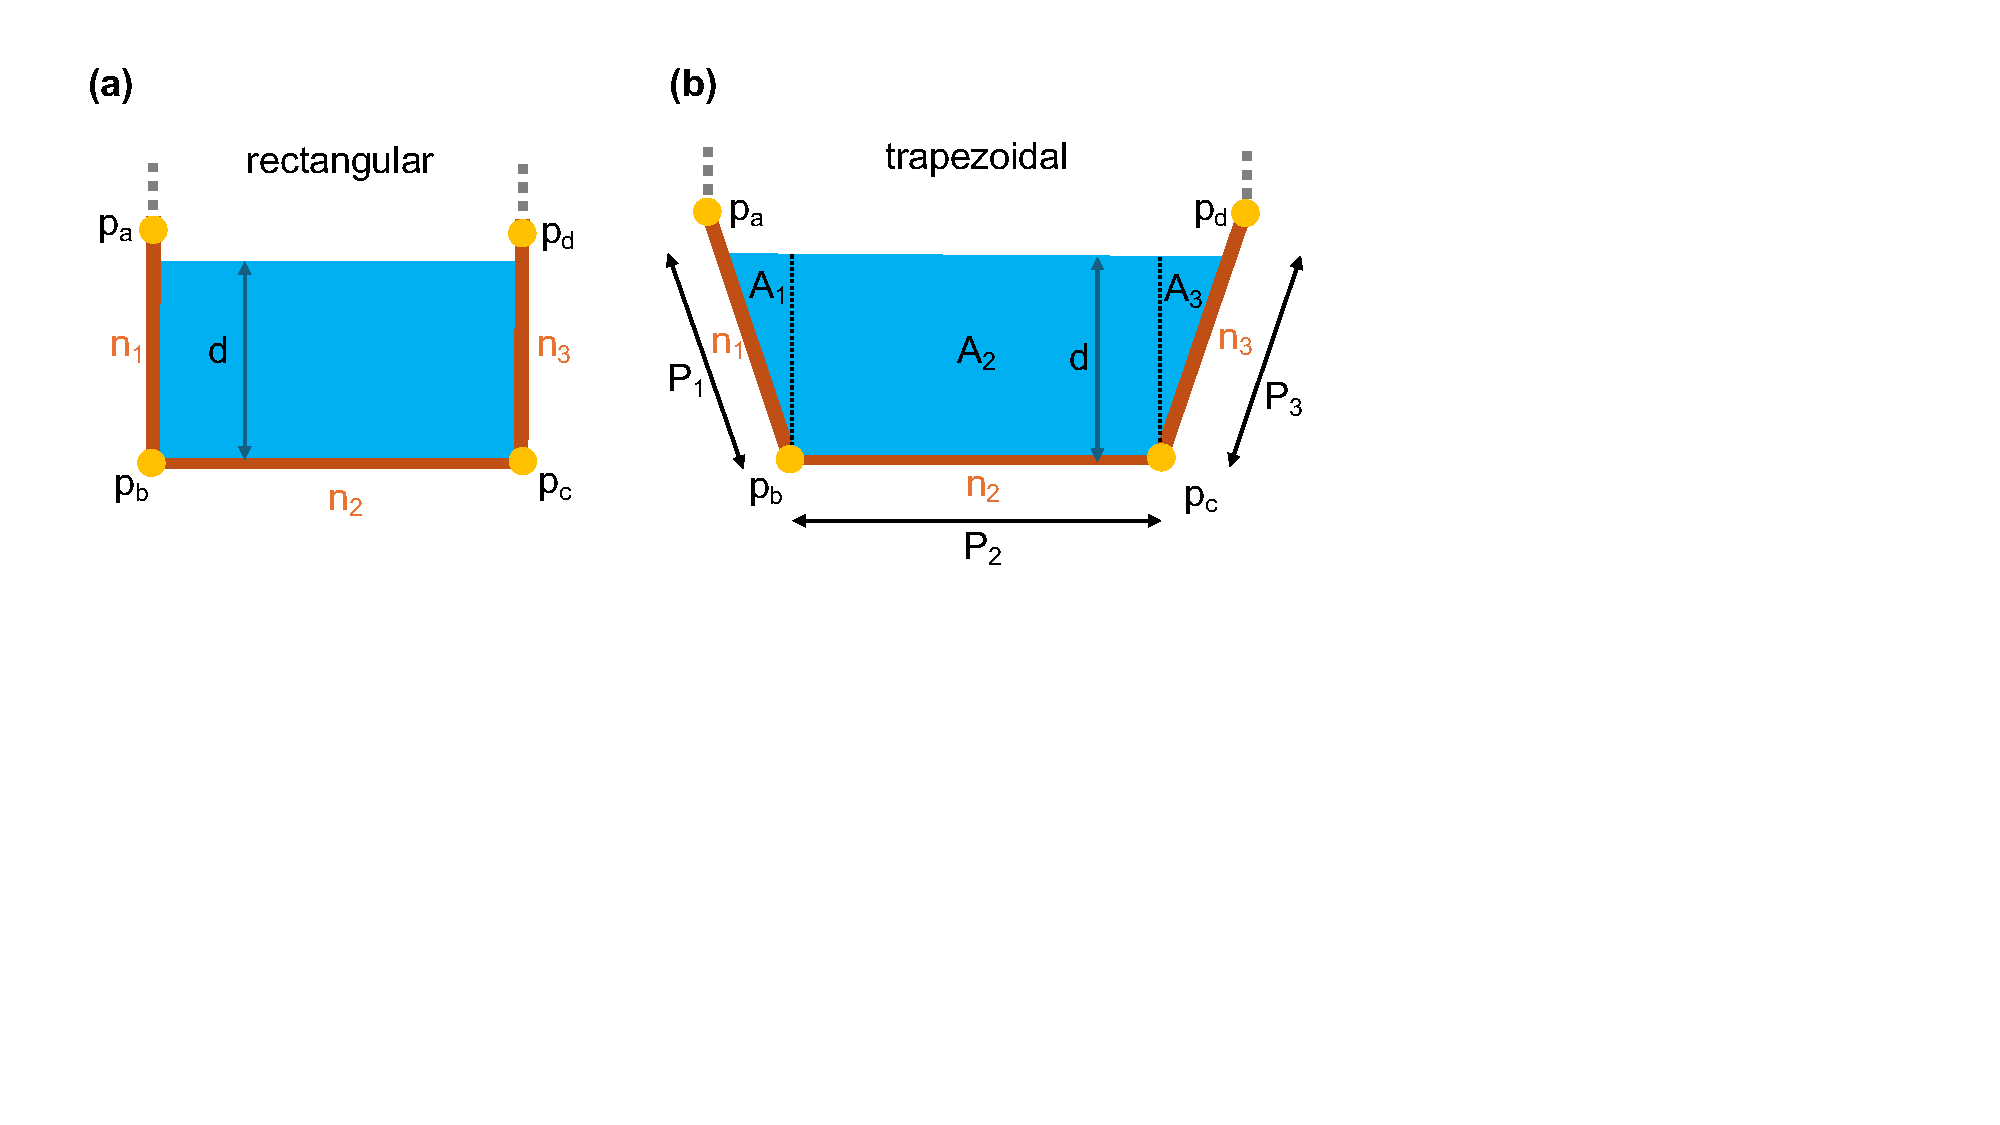
\includegraphics[scale=0.5]{figures/cxs_rough.pdf}
	\caption[Schematic showing different types of channel cross sections with variable roughness.]{Schematic showing different types of cross sections with variable Manning's roughness coefficient: (a) a rectangular cross section defined using four points, and (b) a trapezoidal cross section defined using four points.  The Manning's roughness coefficient is varies by line segment.  If the water surface rises above the channel points, no channel resistance is included for sections above the uppermost points}
	\label{fig:cxs_rough}
\end{figure}


\subsection{Temporal Discretization}
Adaptive time stepping

\subsection{Sources and Sinks}

\subsection{Initial and Boundary Conditions}

A zero-depth-gradient (ZDG) boundary condition can be assigned to any reach to allow from the channel.  Flow out of the channel is calculated as

\begin{equation}
  Q = \frac{1}{n}A R^{2/3} \sqrt{S_0}
\end{equation}


\section{Integration into MODFLOW 6}

The epsilon used for derivative calculation must be small.  1.D-8 was working well until we tried the one-dimensional problem with tiny cells (200,000 cells).  With 1.D-8, a floating point exception was encountered in the dot product as part of the bicgstab calculation.  When this value was reduced to 1.D-12, the program worked as expected.

\section{Examples}

% Ideally, each example should be written up following a similar template.  A possible template is
% background
% purpose of the test
% expectation
% problem description
% results

\subsection{One-Dimensional Channel and Overland Flow}

% background
To ensure that numerical models are working properly, results from numerical simulations are commonly compared with results from an analytical solution.  To demonstrate and test the SWF Model, an analytical solution was developed for simple one-dimensional steady flow.  An analytical solution can be obtained for the following mathematical governing equation

\begin{equation}
  \frac{\partial h}{\partial t} = \frac{\partial}{\partial x} 
  \left ( \frac{h^{5/3}}{n \left | \frac{\partial h}{\partial x} \right |^{1/2}} 
  \frac{\partial h}{\partial x} \right ) = 0 .
  \label{eqn:gov_1d}
\end{equation}

\noindent Equation~\ref{eqn:gov_1d} describes flow for a hydraulically wide rectangular channel, in which the wetted perimeter is equal to the channel width, and the bottom is flat with an elevation of zero.  Under these conditions, the water surface elevation $h$ is equal to the water depth $d$.  For flow between two locations, $x_0$ and $x_1$, with prescribed stages of $h_0$ and $h_1$, respectively, the analytical solution for $h$ as a function of $x$ is

\begin{equation}
  h = \left [ \left (1 - \rho \right ) h^{\frac{13}{3}}_{0} + \rho h^{\frac{13}{3}}_{1} \right ]^{\frac{3}{13}} ,
  \label{eqn:asoln_1d}
\end{equation}

\noindent where

\begin{equation}
  \rho \equiv \frac{x - x_0}{x_1 - x_0} .
  \label{eqn:rho_defined_x}
\end{equation}

\noindent Equation~\ref{eqn:asoln_1d} can be solved easily to produce steady channel stage profiles for comparison with model results.

Under these conditions the flow rate $Q$ can be calculated as

\begin{equation}
  Q = \frac{1}{n} \left ( 
    \frac{3}{13}
    \frac{h^{\frac{13}{3}}_{0} - h^{\frac{13}{3}}_{1}}{x_1 - x_0}
  \right )^{1/2}.
  \label{eqn:q_calc}
\end{equation}


% purpose and expectation
In this example, a simple one-dimensional numerical model is used to simulate flow and the water surface profile between two prescribed stage boundaries.  Results from the numerical model should be in agreement with the analytical solution.  Some minor differences are expected due to upstream weighting and discretization errors in the numerical model.  These differences between the numerical model and the analytical solution should decrease with increases in model grid resolution.

%problem description
One dimensional steady flow is simulated using two different approaches.  The DISV1D discretization is used for the first approach to represent flow in a channel.  The DIS2D discretization, with a single row, is used to represent flow in overland conditions.  In this example, a model domain extending 110 km in the x direction is divided into 501 cells.  Prescribed stage conditions are assigned to the first and last cells.  A stage value of 10.0 m is assigned to the first cell and a value of 1.0 m is assigned to the last cell.  Steady conditions are solved using a stage tolerance of $10^{-8}$ m.

%results
The comparison between the analytical solution (equation~\ref{eqn:asoln_1d}) and the channel and overland flow models are shown in figure~\ref{fig:oned-results}.  The upper plot shows the stage profile (for every tenth point) and the close agreeement between the analytical and numerical solutions.  Although there is good agreement between the numerical models and the analytical solution, the lower plot shows that maximum errors between the models and the analytical solution are about 0.4 m.  This error in the numerical models is due to spatial discretization.  An increase in spatial resolution results in a better match with the analytical solution.  Using equation~\ref{eqn:q_calc} the flow under these conditions is 0.212805 $m^3/s$.  The simulated flow for the channel and overland models is in error by about 0.3 percent. Simulated flow for the channel and overland models 0.213465 and 0.213428 $m^3/s$, respectively.  

\begin{figure}[h!tbp]
	\centering
	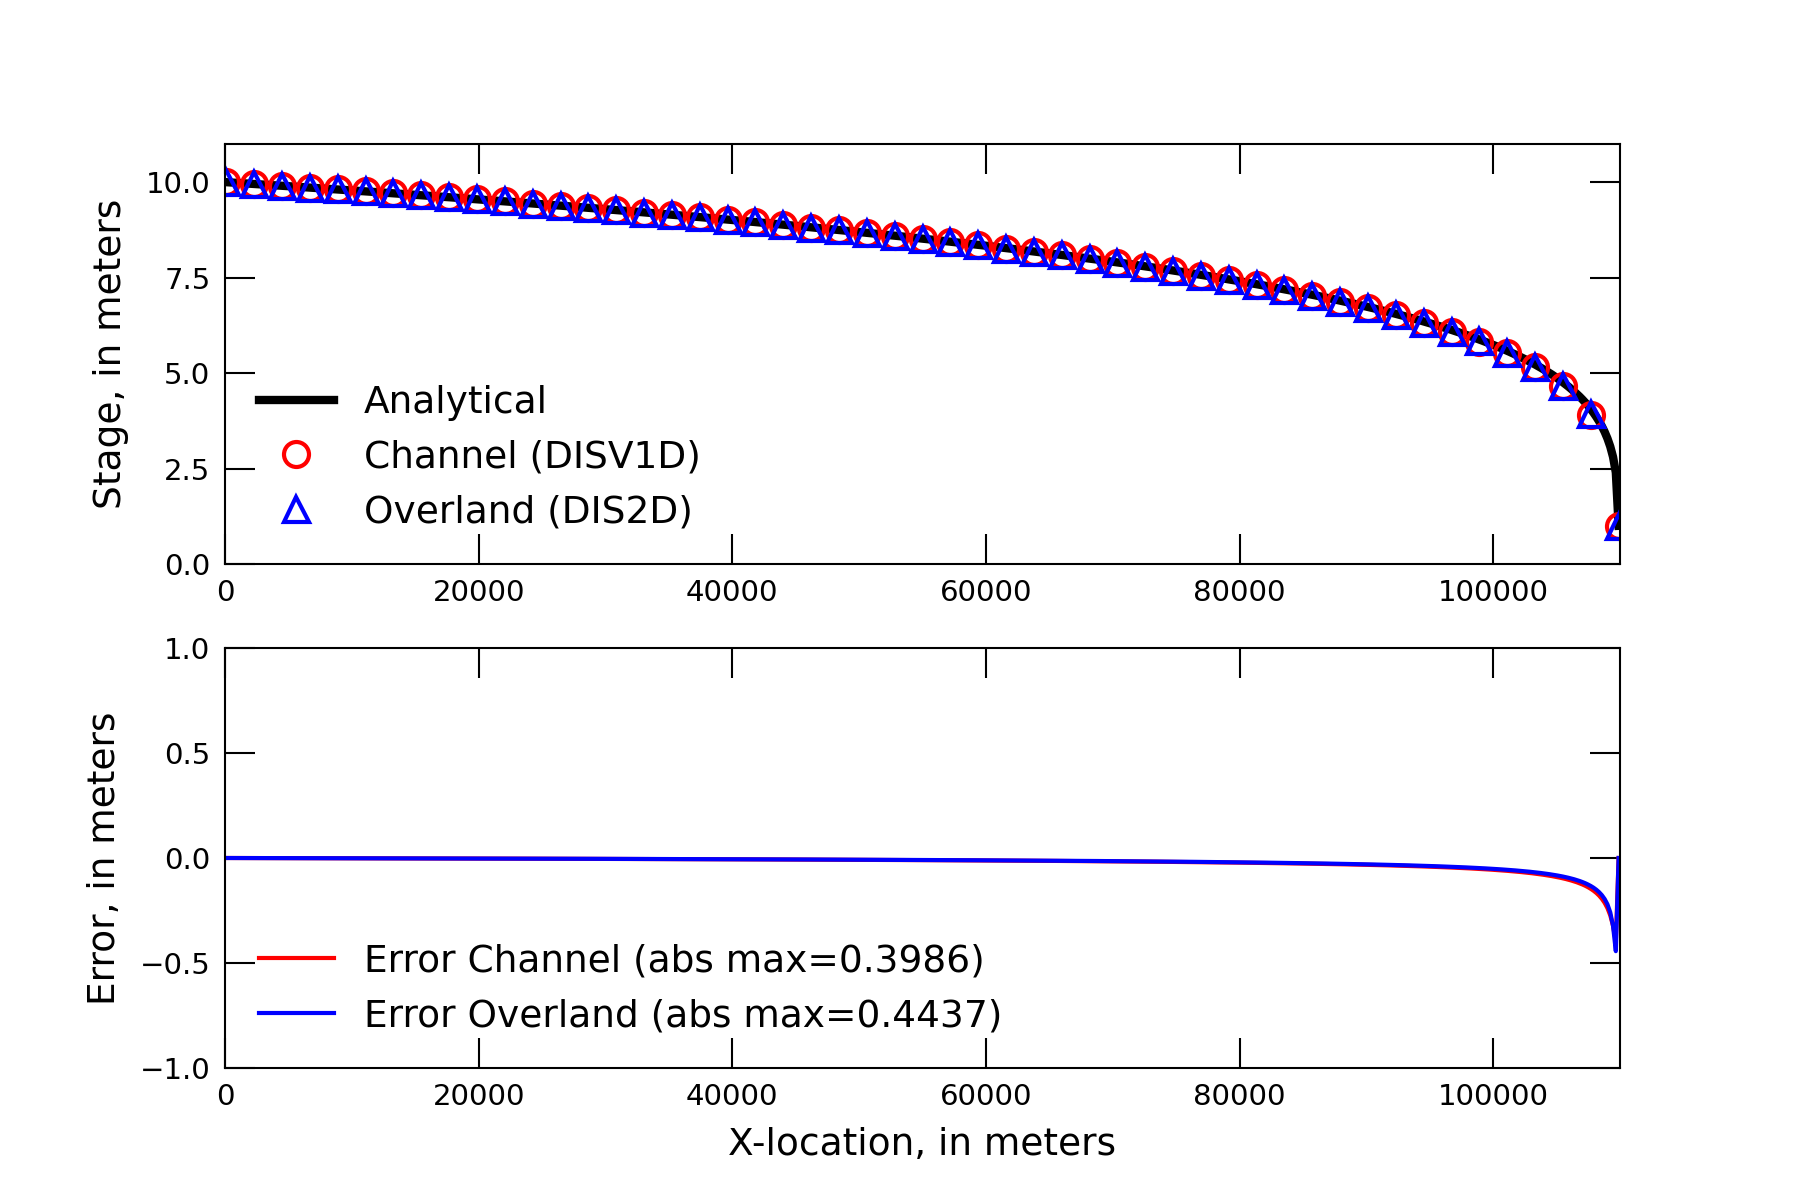
\includegraphics[scale=1.0]{figures/oned.png}
	\caption[Results for one-dimensional flow.]{Results for one-dimensional flow.  Two different Surface Water Flow (SWF) Models are shown.  The channel model represents flow using the one-dimensional DISV1D discretization.  The overland model represents flow using the two-dimensional DIS2D discretization with a single row.}
	\label{fig:oned-results}
\end{figure}


\subsection{Axisymmetric Overland Flow}

The axisymmetric flopy problem developed by~\cite{lal2001}, and used by~\cite{hughes2015} to test the SWR Process for MODFLOW-2005, is used to test the SWF Model for MODFLOW 6.  The problem is based on the transient decay of a circular mound of surface water.

\begin{figure}[h!tbp]
	\centering
	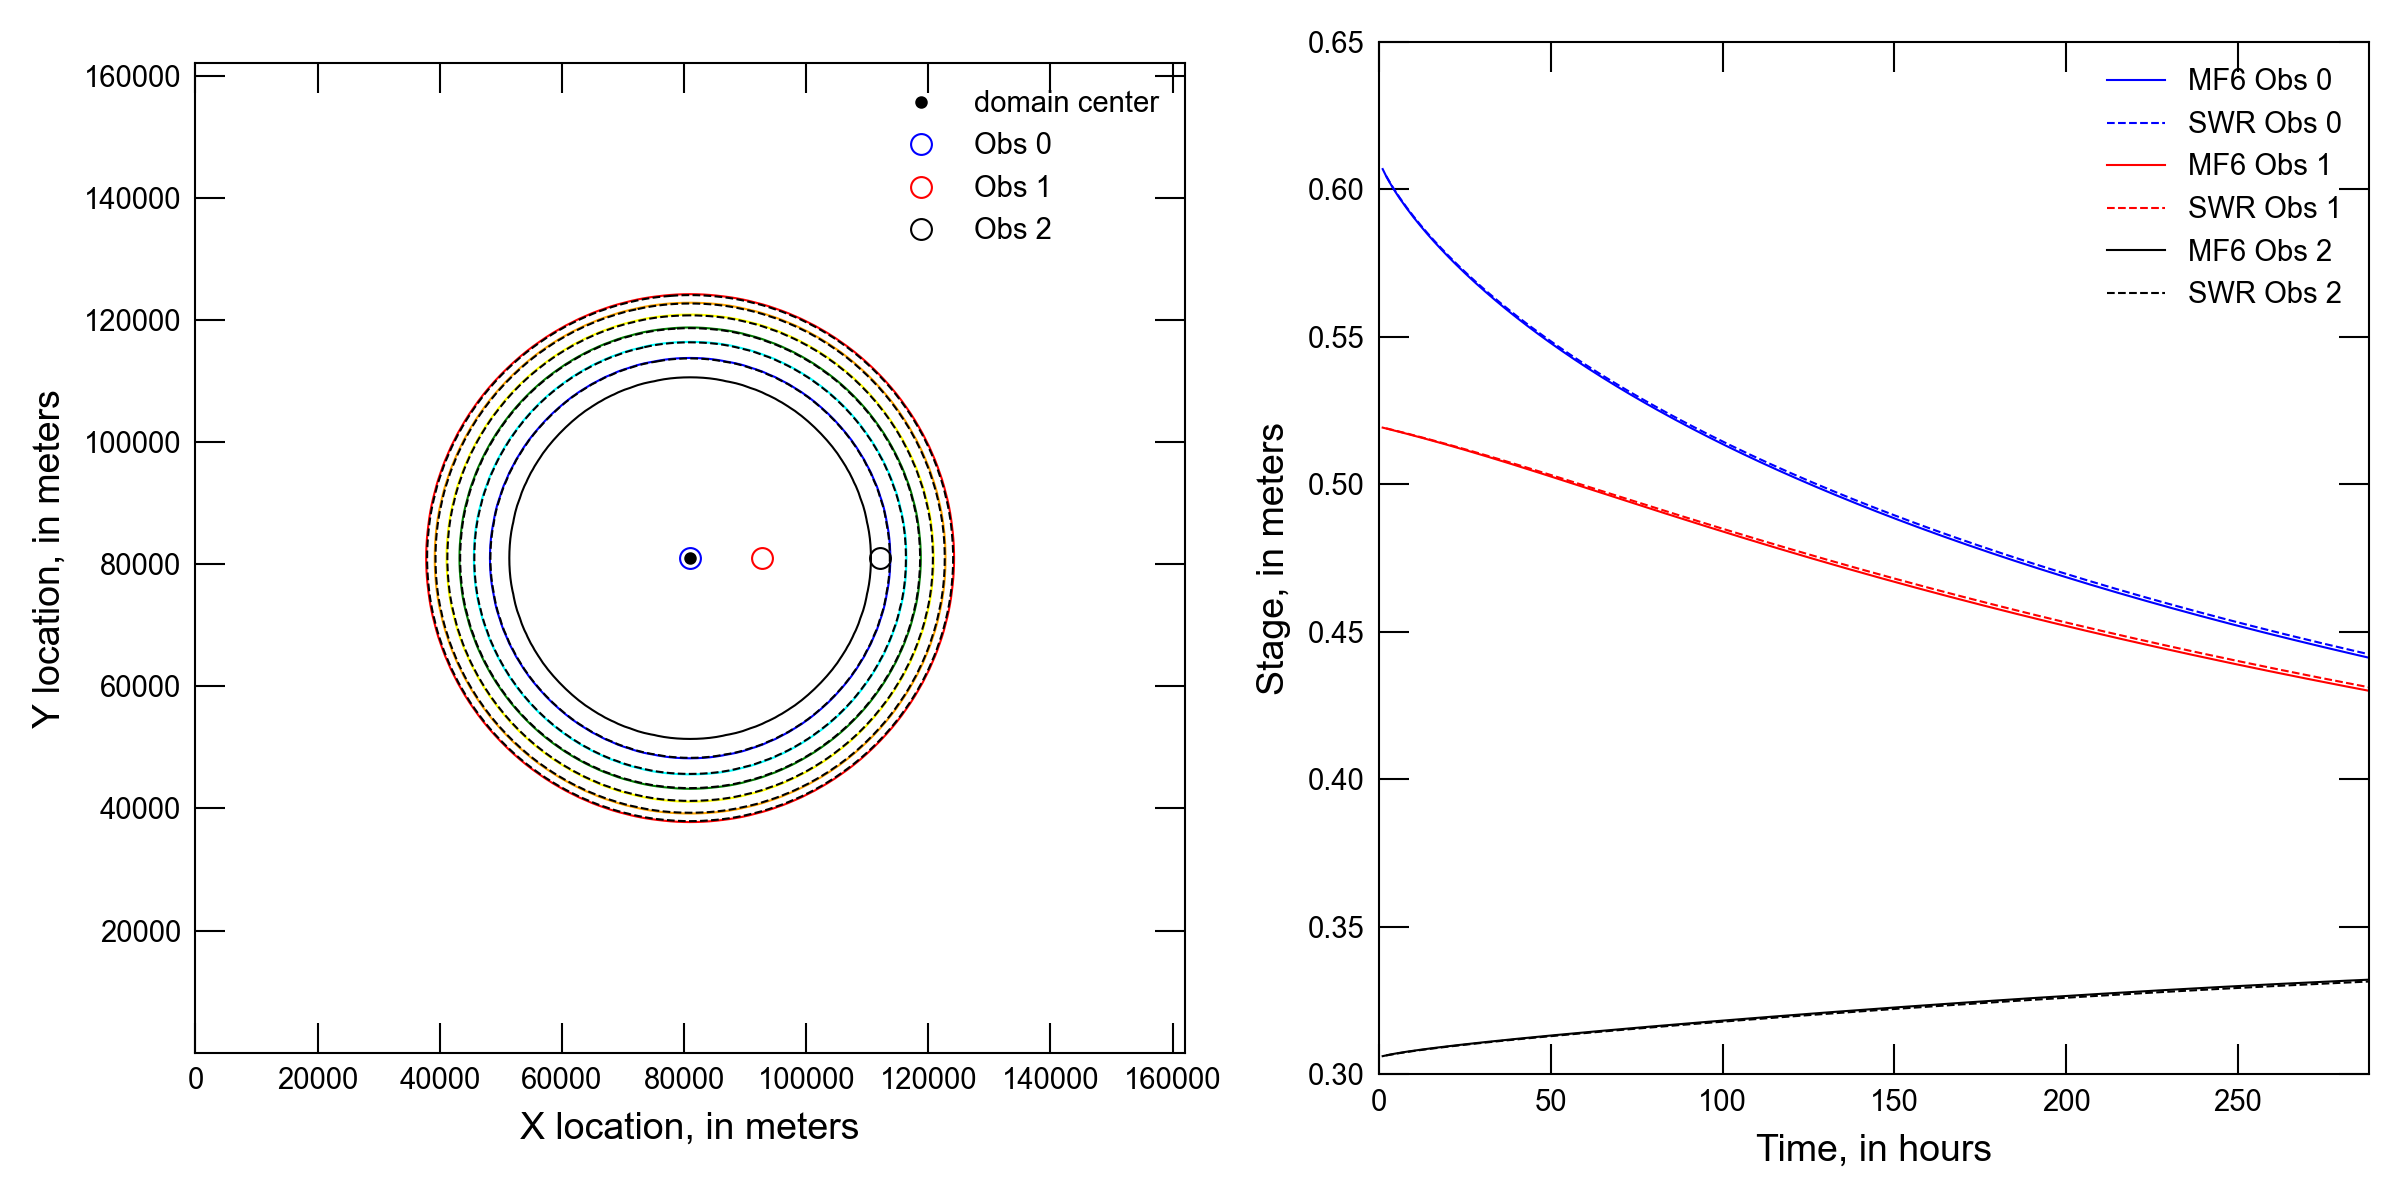
\includegraphics[scale=0.70]{figures/axi-results.png}
	\caption[Simulation results for the axisymmetric overland flow problem.]{Simulation results for the axisymmetric overland flow problem.}
	\label{fig:axi-results}
\end{figure}

\subsection{Radial Flow}
If the bed is level at elevation $z = 0$ and the depth is equal to the stage ($d = h$), then the governing equation for one-dimensional radial surface water flow is

\begin{equation}
  \frac{\partial h}{\partial t} = \frac{1}{r} \frac{\partial}{\partial r} 
  \left (r \frac{h^{5/3}}{n \left | \frac{\partial h}{\partial r} \right |^{1/2}} 
  \frac{\partial h}{\partial r} \right ) = 0 .
\end{equation}

\noindent For flow between two prescribed stage boundaries, with stages of $h_0$ and $h_1$ at radial distances of $r_0$ and $r_1$, respectively, the analytical solution is

\begin{equation}
  h = \left [ \left (1 - \rho \right ) h^{\frac{13}{3}}_{0} + \rho h^{\frac{13}{3}}_{1} \right ]^{\frac{3}{13}} ,
  \label{eqn:soln_ss}
\end{equation}

\noindent where

\begin{equation}
  \rho \equiv \frac{\frac{1}{r_{0}} - \frac{1}{r}}{\frac{1}{r_{0}} - \frac{1}{r_{1}}} .
  \label{eqn:rho_defined}
\end{equation}

Radial flow is simulated with the SWF Model using a regular grid consisting of 151 rows and 151 columns.  Radial flow is also simulated using the voronoi model grid shown in figure xxx.


\subsection{Tilted V-Catchment}

The MODFLOW 6 SWF Model was used to simulate the tilted V-catchment problem described by \cite{digiammarco1996}.  This tilted V-catchment problem has been used by~\cite{VanderKwaak1999},~\cite{panday2004} and by~\cite{hughes2015}, for example, to test numerical models of two-dimensional overland in response to a rainfall event.

The configuration of the tilted V-catchment is shown in Figure~\ref{fig:vcatch-surface}.  The left and right sides of the domain consist of sloping flat planes.  The flat planes are tilted to the south and toward the middle of the domain, forming a V-shaped catchment.  A slope of 0.05 is used for the x direction, and a slope of 0.02 is used for the y direction.  Located between the two sloping planes is a 20-m wide stream channel that slopes from north to south.  Two different Mannings roughness coefficients are used.  A value of 0.015 is assigned to the sloping planes and a value of 0.15 is assigned to the stream channel.  These values are not realistic, in that roughness coefficients are generally lower within a stream channel compared to sloping surfaces, but they were selected as a difficult test for simulating overland flow.  A zero-depth gradient boundary condition assigned as the southernmost part of the stream provides the sole outlet for the domain.

\begin{figure}[h!tbp]
	\centering
	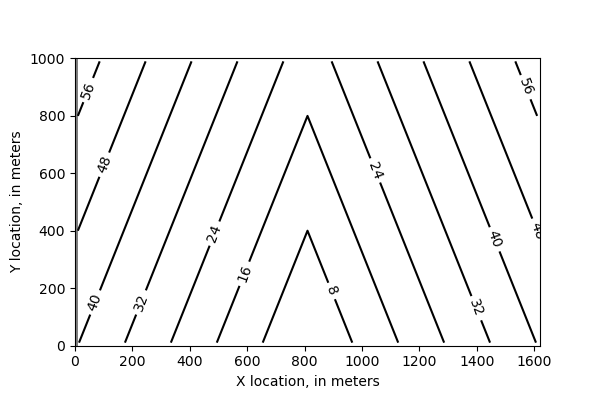
\includegraphics[scale=0.75]{figures/vcatch-surface.png}
	\caption[Configuration of the tilted v-catchment example.]{Configuration of the tilted v-catchment example.  Contours represent land surface.  A slope of 0.05 is used for the x direction, and a slope of 0.02 is used for the y direction.  A 20-m wide stream channel, shown in gray, slopes from north to south.}
	\label{fig:vcatch-surface}
\end{figure}

The domain is discretized into a regular model grid consisting of 50 rows and 81 columns.  Each cell is square with a dimension of 20 m.  Rainfall is uniformly applied to the domain at a rate of $3 \times 10^{-6}$ for a period of 90 minutes.  A second 90-minute period with no rainfall is also represented to simulate drainage of the domain in response to the rainfall event.  Following the settings used by~\cite{panday2004} adaptive time stepping is used with an inital time step of 5 s and a maximum time step of 100 s.  Time steps increase or decrease by a factor of two in response to solver behavior.

Results from the MODFLOW 6 SWF Model simulation are compared in Figure~\ref{fig:vcatch} with the simulations results of~\cite{digiammarco1996},~\cite{VanderKwaak1999},~\cite{panday2004} and~\cite{hughes2015}.  In general, the model results from MODFLOW 6 compare favorably with the results from these other models; however, rates of simulated outflow from the MODFLOW 6 simulation rise and fall more quickly than for the other models.

\begin{figure}
	\centering
	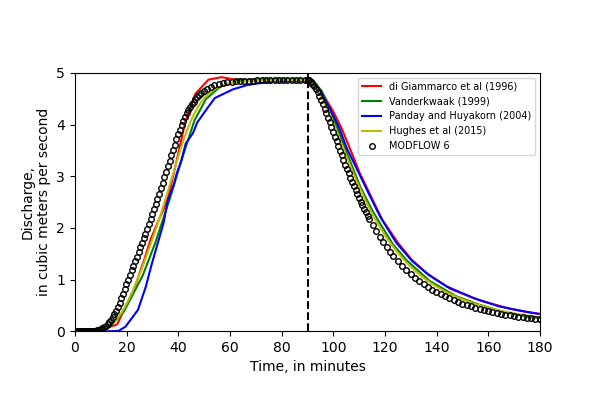
\includegraphics[scale=0.75]{figures/vcatch-results.png}
	\caption[Simulated discharge for the tilted v-catchment example.]{Simulated discharge for the tilted v-catchment example.  Dashed blue line separates the first 90-minute period with rainfall from the second 90-minute period with no rainfall.}
	\label{fig:vcatch}
\end{figure}

\bibliographystyle{plain}
\bibliography{swfref} 

\end{document}